\section{Sensitivity Analysis}
\label{sec:sensitivity_analysis}
We refined the CycleGAN performance by tuning two critical hyperparameters: input patch size and cycle-consistency loss weight.

\subsection{Impact of Patch Size}
The input patch size defines the generator's receptive field.
We evaluated four resolutions: $64 \times 64$, $128 \times 128$, $256 \times 256$, and $512 \times 512$ pixels (see visual comparisons in Figure~\ref{fig:patch_size_comparison}).

\begin{figure}[htbp]
    \centering
    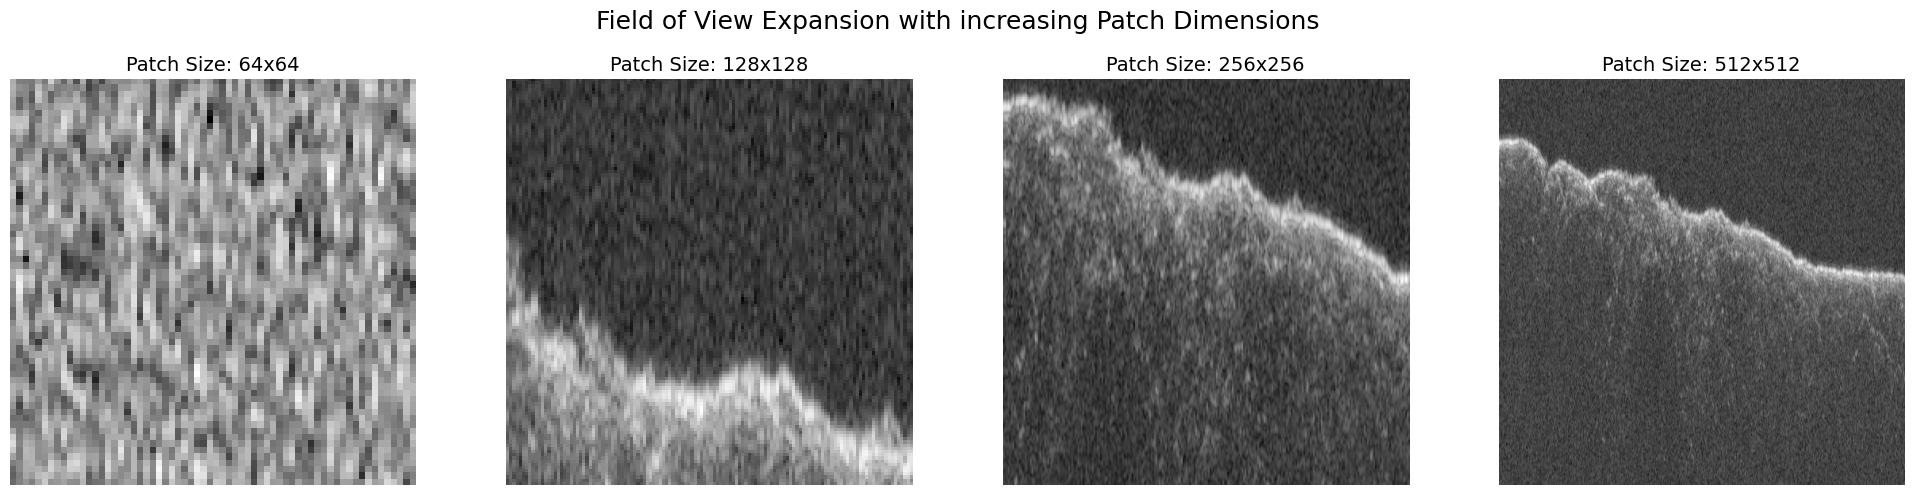
\includegraphics[width=\textwidth]{images/example_plots/ID_01970402/varying_patch_sizes}
    \caption{Field of View expansion with increasing patch dimensions. From left to right: $64\times64$, $128\times128$, $256\times256$, and $512\times512$ pixels, all extracted from the same radargram location. At $64\times64$, the receptive field is too narrow to resolve any coherent stratigraphic structure, yielding a texture-only view devoid of geological context. At $128\times128$, the principal surface echo and the transition into the subsurface noise floor are both visible, providing sufficient context for training. Larger patches ($256\times256$ and $512\times512$) progressively include the deep, signal-poor region of the radargram, diluting the informative content and increasing memory overhead without a corresponding gain in structural detail.}
    \label{fig:patch_size_comparison}
\end{figure}

Small patches ($64 \times 64$) restrict the effective spatial context, or Field of View (FoV).
The model fails to capture the continuity of long subsurface reflectors, causing layers to abruptly end at patch boundaries.

Conversely, $512 \times 512$ patches consume excessive VRAM, forcing a batch size of 1.
This causes noisy gradients and unstable training.
Moreover, large patches include deep, signal-poor regions that provide no useful features.

We identified $128 \times 128$ as the optimal size.
It captures essential geological structures (horizontal layers and hyperbolic diffractions) while maintaining a stable batch size.
Physically, 128 pixels cover $\approx 2$ km of depth, providing enough context for shallow anomalies without wasting computation.

\subsection{Weighting the Cycle-Consistency Loss}
The parameter $\lambda_{cycle}$ controls the contribution of the cycle-consistency loss relative to the adversarial loss.
It dictates the penalty for altering the image's structural content:

$$L_{total}=L_{GAN}+\lambda_{cycle}L_{cyc}$$

Through empirical validation on the validation set, we determined that $\lambda_{cycle}=10.0$ provides the optimal balance. 

A low $\lambda_{cycle}$ gives the generator excessive freedom.
While the model generates plausible radar textures, it geometrically distorts or entirely fabricates subsurface layers, destroying the physical validity of the synthetic data.

Conversely, an excessively high $\lambda_{cycle}$ constrains the generator to perform an identity mapping.
The model perfectly preserves the geometry but fails to inject the requisite speckle noise and thermal clutter, defeating the purpose of domain adaptation.

A weighting of 10.0 is strong enough to enforce the strict preservation of the principal stratigraphic horizons.
Simultaneously, it allows the adversarial network to successfully overlay the high-frequency noise texture characteristic of the SHARAD sensor.

